% Options for packages loaded elsewhere
\PassOptionsToPackage{unicode}{hyperref}
\PassOptionsToPackage{hyphens}{url}
%
\documentclass[
]{article}
\usepackage{lmodern}
\usepackage{amssymb,amsmath}
\usepackage{ifxetex,ifluatex}
\ifnum 0\ifxetex 1\fi\ifluatex 1\fi=0 % if pdftex
  \usepackage[T1]{fontenc}
  \usepackage[utf8]{inputenc}
  \usepackage{textcomp} % provide euro and other symbols
\else % if luatex or xetex
  \usepackage{unicode-math}
  \defaultfontfeatures{Scale=MatchLowercase}
  \defaultfontfeatures[\rmfamily]{Ligatures=TeX,Scale=1}
\fi
% Use upquote if available, for straight quotes in verbatim environments
\IfFileExists{upquote.sty}{\usepackage{upquote}}{}
\IfFileExists{microtype.sty}{% use microtype if available
  \usepackage[]{microtype}
  \UseMicrotypeSet[protrusion]{basicmath} % disable protrusion for tt fonts
}{}
\makeatletter
\@ifundefined{KOMAClassName}{% if non-KOMA class
  \IfFileExists{parskip.sty}{%
    \usepackage{parskip}
  }{% else
    \setlength{\parindent}{0pt}
    \setlength{\parskip}{6pt plus 2pt minus 1pt}}
}{% if KOMA class
  \KOMAoptions{parskip=half}}
\makeatother
\usepackage{xcolor}
\IfFileExists{xurl.sty}{\usepackage{xurl}}{} % add URL line breaks if available
\IfFileExists{bookmark.sty}{\usepackage{bookmark}}{\usepackage{hyperref}}
\hypersetup{
  pdftitle={Protein-Protein Interactions},
  pdfauthor={Tianyi Shi},
  hidelinks,
  pdfcreator={LaTeX via pandoc}}
\urlstyle{same} % disable monospaced font for URLs
\usepackage[margin=1in]{geometry}
\usepackage{longtable,booktabs}
% Correct order of tables after \paragraph or \subparagraph
\usepackage{etoolbox}
\makeatletter
\patchcmd\longtable{\par}{\if@noskipsec\mbox{}\fi\par}{}{}
\makeatother
% Allow footnotes in longtable head/foot
\IfFileExists{footnotehyper.sty}{\usepackage{footnotehyper}}{\usepackage{footnote}}
\makesavenoteenv{longtable}
\usepackage{graphicx}
\makeatletter
\def\maxwidth{\ifdim\Gin@nat@width>\linewidth\linewidth\else\Gin@nat@width\fi}
\def\maxheight{\ifdim\Gin@nat@height>\textheight\textheight\else\Gin@nat@height\fi}
\makeatother
% Scale images if necessary, so that they will not overflow the page
% margins by default, and it is still possible to overwrite the defaults
% using explicit options in \includegraphics[width, height, ...]{}
\setkeys{Gin}{width=\maxwidth,height=\maxheight,keepaspectratio}
% Set default figure placement to htbp
\makeatletter
\def\fps@figure{htbp}
\makeatother
\setlength{\emergencystretch}{3em} % prevent overfull lines
\providecommand{\tightlist}{%
  \setlength{\itemsep}{0pt}\setlength{\parskip}{0pt}}
\setcounter{secnumdepth}{5}
\newlength{\cslhangindent}
\setlength{\cslhangindent}{1.5em}
\newenvironment{cslreferences}%
  {\setlength{\parindent}{0pt}%
  \everypar{\setlength{\hangindent}{\cslhangindent}}\ignorespaces}%
  {\par}

\title{Protein-Protein Interactions}
\author{Tianyi Shi}
\date{2020-11-18}

\begin{document}
\maketitle

{
\setcounter{tocdepth}{2}
\tableofcontents
}
\textbf{How and why do proteins form specific complexes with each other? How can such protein-protein interactions (PPIs) be investigated experimentally, and which problems are associated with designing small molecules to disrupt PPIs?}

\hypertarget{introduction}{%
\section{Introduction}\label{introduction}}

Specific protein-protein interactions (PPIs) are critical to numerous biological processes, including cell-cell recognition, immune response, and signal transduction. An understanding of PPIs helps to elucidate the detailed roles and to predict the behaviour of proteins in a physiological context. On the other hand, disruption of PPIs is a target of structure-based drug design.

\hypertarget{properties-of-ppi}{%
\section{Properties of PPI}\label{properties-of-ppi}}

\hypertarget{reversibility}{%
\subsection{Reversibility}\label{reversibility}}

Protein-protein interactions can be stable (permanent) or transient. Stable interactions are involved in the assembly of proteins made of multi-subunit complexes such as haemoglobin, which non-reversible in normal physiological conditions. Transient interactions, on the other hand, are reversible, and it is this property that make them act like molecular switches that play versatile roles in controlling cellular processes.

\hypertarget{properties-of-the-binding-interfaces}{%
\subsection{Properties of the Binding Interfaces}\label{properties-of-the-binding-interfaces}}

Protein-protein interaction interfaces often have a large surface area (1000-2000 Å\textsuperscript{2}) and are relatively flat compared to the deep cavities that typically bind small molecules.
On a binding interface, some residues, known as ``hotspots'', contribute more significantly than other residues.

\hypertarget{kd}{%
\subsection{Kinetics and Thermodynamics}\label{kd}}

Reversible PPIs have two important parameters: affinity and specificity. While affinity ranges from as low as millimolar to as high as femtomolar, it is important that the specificity, i.e.~the relative affinity of a protein to its cognate binding partner compared to non-cognate ones, is high.

Reversible PPIs can the considered as a simple balance of association and dissociation reactions, with rate constants being \(k_{\text{on}}\) and \(k_{\text{off}}\).

\[
\text{A+B}\mathrel{\mathop{\rightleftarrows}^{k_{\text{on}}}_{k_{\text{off}}}} \text{AB}
\]

The affinity is usually defined by:

\[
K_d = \dfrac{\text{[A][B]}}{\text{[AB]}} = \dfrac{k_{\text{off}}}{k_{\text{on}}}
\]

where \texttt{{[}A{]}}, \texttt{{[}B{]}}, and \texttt{{[}AB{]}} are the concentrations of each species at equilibrium.

\hypertarget{studying-ppis}{%
\section{Studying PPIs}\label{studying-ppis}}

\hypertarget{determine-kd}{%
\subsection{\texorpdfstring{Determining K\textsubscript{d} (and rate constants)}{Determining Kd (and rate constants)}}\label{determine-kd}}

There are three experimental methods commonly used for studying thermodynamics and kinetics of PPIs (the frequent tasks are determining \(K_\text{d}\) and rate constants), all assuming the simple single-step association-dissociation model (Section \ref{kd}).

\hypertarget{surface-plasmon-resonance-spr}{%
\subsubsection{Surface Plasmon resonance (SPR)}\label{surface-plasmon-resonance-spr}}

Surface plasmon resonance (Figure \ref{fig:spr}) can be used to measure both \(K_\text{d}\) and \(k_\text{on}\) and \(k_\text{off}\) rates. How \(K_\text{d}\) can be calculated is explained in Equation \eqref{eq:spr-kd}.



\begin{figure}
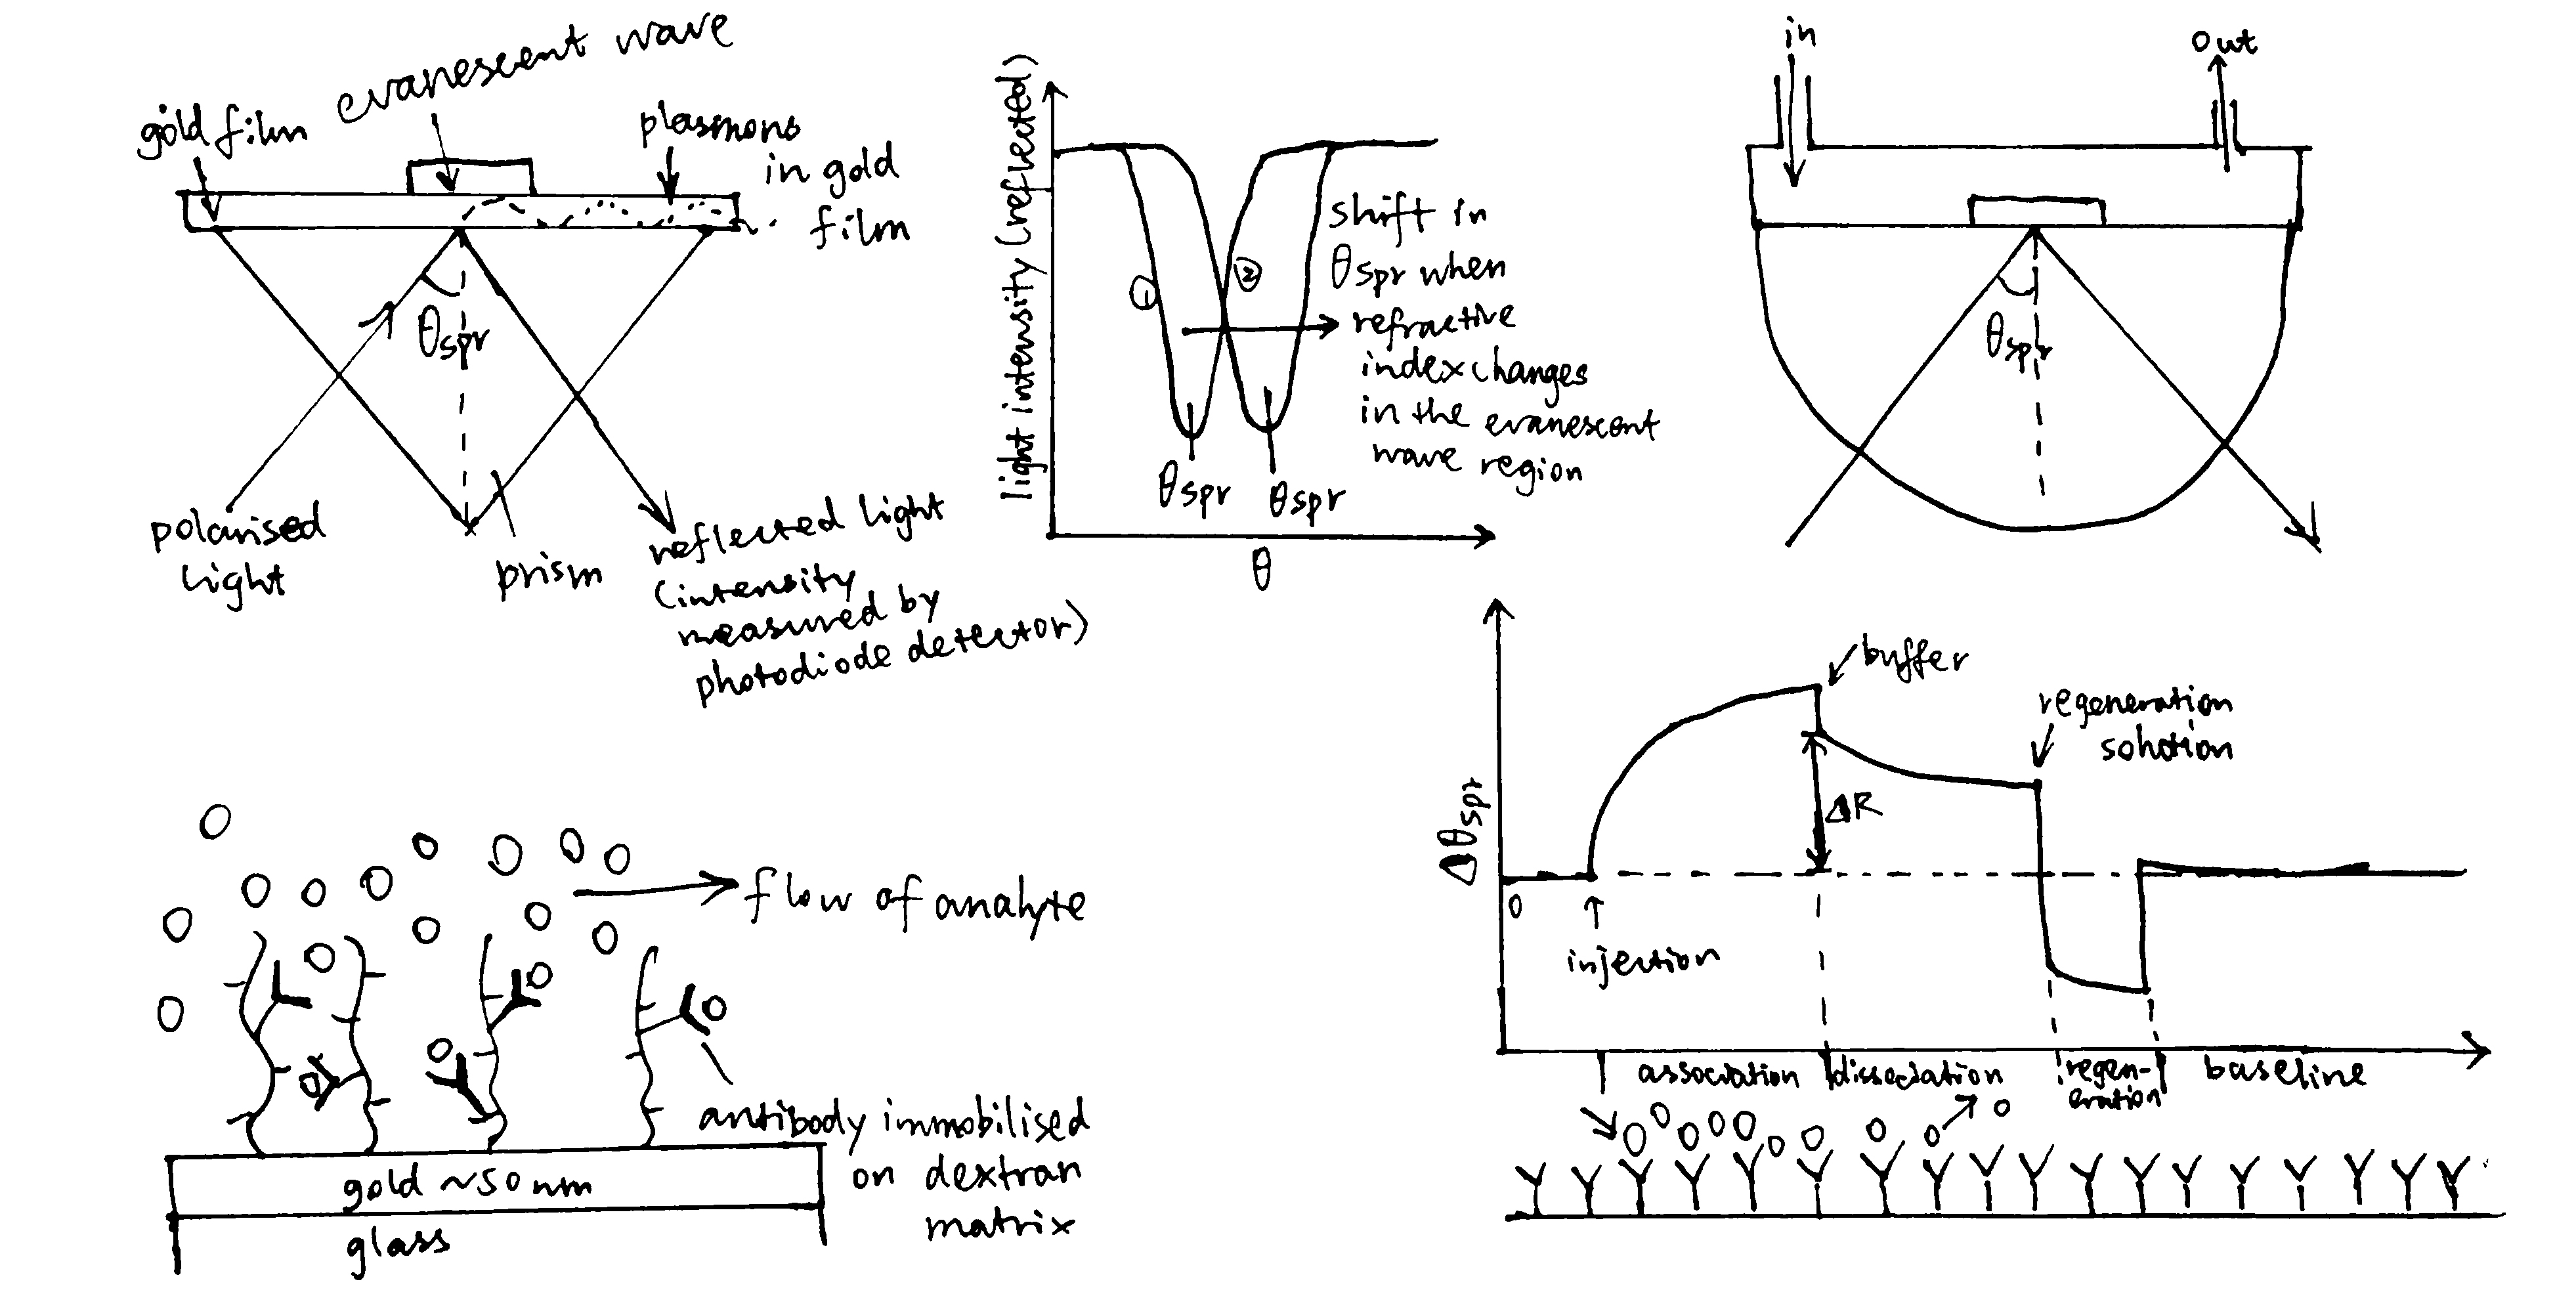
\includegraphics[width=1\linewidth]{../img/spr} \caption{A surface plasmon is an electron oscillation generated at a surface interface between a metal and a dielectric. A plasmon resonance occurs when EM wave in visible light couples optimally with the oscillating electrons in the metal, and this results in a maximal reduction in the reflected light intensity. The resonance angle, \(\theta_\text{spr}\), is found by changing the angle of incidence of the light beam, giving a dip in a plot of intensity against angle. \(\Delta\theta_\text{spr}\) is sensitive to changes in the refractive index of the medium near the metal surface and this is a measure of the mass change at the sensor surface (in the evanescent region). In an SPR experiment, the protein acting as the ``bait'' is immobilised on the sensor surface, and a the analyte containing the other protein (acting as the ``prey'') is passed through the cell. If binding occurs between the two proteins, \(\Delta\theta_\text{spr}\) would increase. Then, non-specific binding is washed off by buffer, and \(\Delta\theta_\text{spr}\) would decrease and \(\Delta\theta_\text{spr}\). Finally, regeneration solution is applied to remove all binding and reset \(\Delta\theta_\text{spr}\) to zero.}\label{fig:spr}
\end{figure}

\$\$

\begin{aligned}
\overbrace{k_{\text{on}}\text{[A][B]}}^\text{rate of association} & = \overbrace{k_{\text{off}}\text{[AB]}}^\text{rate of dissociation} \\
k_{\text{on}}\text{[A]([B]}_{\text{max}}-\text{[AB])} & = k_{\text{off}}\text{[AB]} \\
\text{[AB]} & = \dfrac{k_{\text{on}}\text{[A][B]}_{\text{max}}}{k_{\text{on}}\text{[A]} + k_{\text{off}}} \\
\text{[AB]} & = \dfrac{\text{[A][B]}_{\text{max}}}{\text{[A]} + K_{\text{d}}}


\label{eq:spr-kd}
\end{aligned}

\$\$

In the equation, A is the protein in the analyte, whose concentration is kept constant, and B is the immobilised protein. Since the \(\Delta\theta_\text{spr} \propto \text{[AB]}\) (intensity of the signal is proportional to concentration of protein-protein complexes), we can work out \(K_\text{d}\) from our initial concentrations of A and B.

SPR was used in the early kinetic analysis of hGH binding (Wells (1996)).

\hypertarget{fluorescence-anisotropy}{%
\subsubsection{Fluorescence anisotropy}\label{fluorescence-anisotropy}}

Fluorescence anisotropy is based on the phenomenon that, if fluorophores are excited with plane polarized light and the fluorescence is observed through analyzing polarizers, the fluorescence is also polarised.

The fluorescence anisotropy is defined as \(A=\dfrac{I_\parallel - I_\bot}{I_\parallel+2_{\bot}}\), where \(I_\parallel\) and \(I_{\bot}\) are the fluorescence intensities polarised parallel and perpendicular to the direction of the excitation beam. \(A\) is a direct measure of the molecular rotation in solution and can be used to study complex formation, as a macromolecule will rotate more slowly when it is in a complex thatn when it is alone.

Fluorescence anisotropy is more accurate than SPR for measuring ultra-high affinity interactions, and were used to to study ColE DNase-Im interactions (Papadakos, Wojdyla, and Kleanthous (2012)).

\hypertarget{isothermal-titration-calorimetry-itc}{%
\subsubsection{Isothermal titration calorimetry (ITC)}\label{isothermal-titration-calorimetry-itc}}

ITC measures heat changes when a complex is formed at constant temperature.

In ITC, an insulated reaction cell containing protein is kept at a temperature (usually 8\(^\circ\text{C}\) above the environment) which is equal to the temperature of a reference cell, and the reference cell is kept at a constant temperature by a thermostat. Then, increasing amounts of ligand is added into the chamber, and they form complexes with the protein, which can be exothermic or endothermic. The heat change is compensated by a power supply, which can be converted to \(\Delta H\) of the reaction. As more ligands are added, proteins become saturated and \(\Delta H\) approaches zero. The raw data obtained (power supplied to compensate the heat change caused by each addition of ligands) can be integrated and corrected to give a plot of \(\Delta H\) against the molar ratio of the ligand and the protein, and \(\Delta H\), K\textsubscript{d} and stoichiometry can be inferred from the curve (Figure \ref{fig:itc}).

\begin{figure}
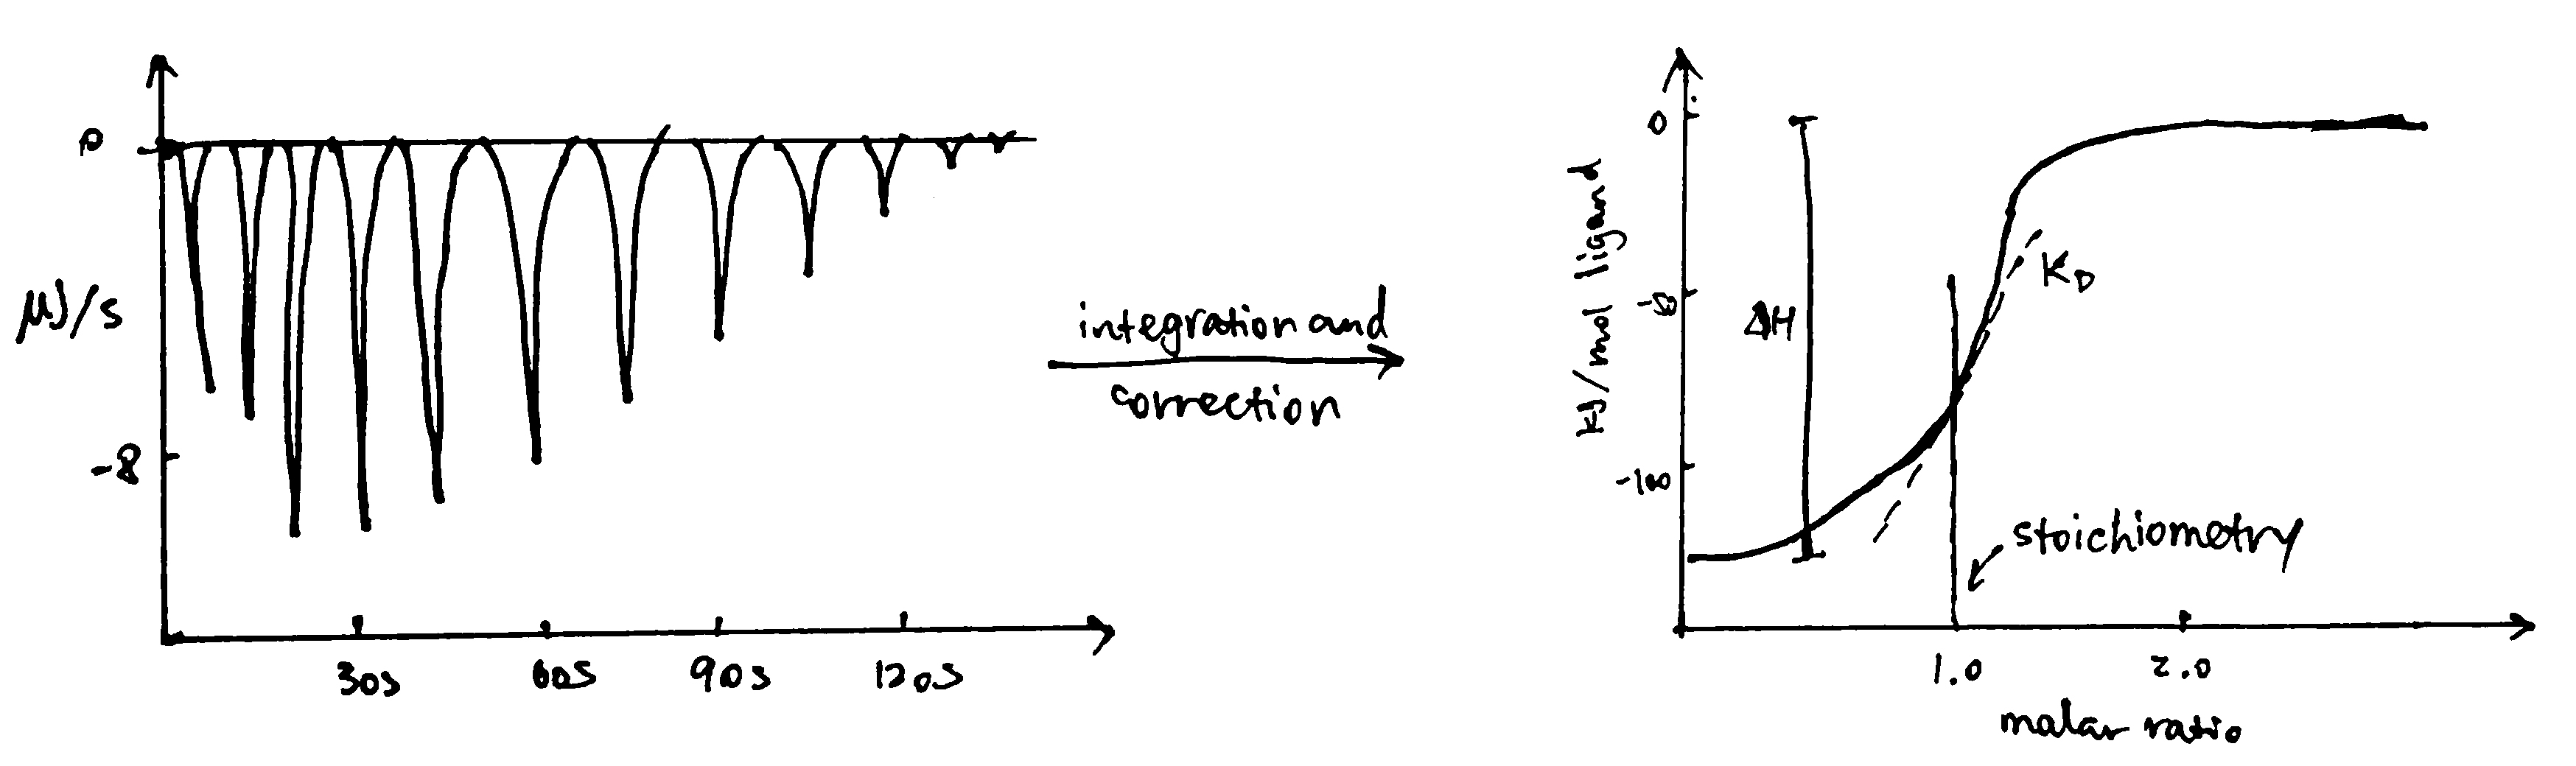
\includegraphics[width=1\linewidth]{../img/itc} \caption{ITC data manipulation}\label{fig:itc}
\end{figure}

\hypertarget{mechanistic-studies}{%
\section{Mechanistic Studies}\label{mechanistic-studies}}

Much knowledge on mechanisms of PPIs came from studies on the interactions between colicin E DNases (ColE) and their immune protein (Im).

\hypertarget{finding-hotspots}{%
\subsection{Finding ``hotspots''}\label{finding-hotspots}}

\hypertarget{alanine-scanning}{%
\subsubsection{Alanine Scanning}\label{alanine-scanning}}

Alanine scanning is a mutagenesis technique in which mutants are made by substituting alanine for each of the residues in a `reactive region', in this case the PPI interface. By comparing the PPI affininy and specificity of each mutant to the wild type, the contribution of each residue in binding can be assessed. However,

\hypertarget{x-ray-crystallography}{%
\subsubsection{X-Ray Crystallography}\label{x-ray-crystallography}}

\hypertarget{nmr}{%
\subsubsection{NMR}\label{nmr}}

Nuclear magnetic resonance is advantageous for characterizing weak PPIs

\hypertarget{mechanisms-of-ppis}{%
\section{Mechanisms of PPIs}\label{mechanisms-of-ppis}}

In addition to the simple model described in Section \ref{kd}, Keeble and Kleanthous (2005) suggested that some relatively low affinity PPIs may be better modelled as a two-step process involving an unstable intermediate, where electrostatics drives the fast first step (supported by strong dependence on ionic strength) and rigid body rotation occurs in the slow second step:

\[
\text{A+B} \mathrel{\mathop{\rightleftarrows}^{k_{1}}_{k_{-1}}} \text{AB}^\text{*} \mathrel{\mathop{\rightleftarrows}^{k_{2}}_{k_{-2}}} \text{AB}
\]

\hypertarget{modularity}{%
\subsection{Modularity}\label{modularity}}

Reichmann et al. (2005)

\hypertarget{references}{%
\section*{References}\label{references}}
\addcontentsline{toc}{section}{References}

\hypertarget{refs}{}
\begin{cslreferences}
\leavevmode\hypertarget{ref-Arkin-2014}{}%
Arkin, Michelle R, Yinyan Tang, and James A Wells. 2014. ``Small-Molecule Inhibitors of Protein-Protein Interactions: Progressing Toward the Reality.'' \emph{Chem Biol} 21 (9): 1102--14. \url{https://doi.org/10.1016/j.chembiol.2014.09.001}.

\leavevmode\hypertarget{ref-Keeble-2005}{}%
Keeble, Anthony H, and Colin Kleanthous. 2005. ``The Kinetic Basis for Dual Recognition in Colicin Endonuclease-Immunity Protein Complexes.'' \emph{J Mol Biol} 352 (3): 656--71. \url{https://doi.org/10.1016/j.jmb.2005.07.035}.

\leavevmode\hypertarget{ref-Papadakos-2012}{}%
Papadakos, Grigorios, Justyna A. Wojdyla, and Colin Kleanthous. 2012. ``Nuclease Colicins and Their Immunity Proteins.'' \emph{Quarterly Reviews of Biophysics} 45 (1): 57--103. \url{https://doi.org/10.1017/S0033583511000114}.

\leavevmode\hypertarget{ref-Reichmann-2005}{}%
Reichmann, D, O Rahat, S Albeck, R Meged, O Dym, and G Schreiber. 2005. ``The Modular Architecture of Protein-Protein Binding Interfaces.'' \emph{Proc Natl Acad Sci U S A} 102 (1): 57--62. \url{https://doi.org/10.1073/pnas.0407280102}.

\leavevmode\hypertarget{ref-Wells-1996}{}%
Wells, J A. 1996. ``Binding in the Growth Hormone Receptor Complex.'' \emph{Proceedings of the National Academy of Sciences} 93 (1): 1--6. \url{https://doi.org/10.1073/pnas.93.1.1}.

\leavevmode\hypertarget{ref-Wienken-2010}{}%
Wienken, Christoph J., Philipp Baaske, Ulrich Rothbauer, Dieter Braun, and Stefan Duhr. 2010. ``Protein-Binding Assays in Biological Liquids Using Microscale Thermophoresis.'' \emph{Nature Communications} 1 (1): 100. \url{https://doi.org/10.1038/ncomms1093}.
\end{cslreferences}

\end{document}
